\documentclass{sig-alternate}
\usepackage{url}
\usepackage[flushleft]{threeparttable}
\begin{document}

\title{A Case Study in Preserving a High Energy Physics Application}
\author{
Haiyan Meng, Matthias Wolf, Peter Ivie, Anna Woodard, Michael Hildreth, and Douglas Thain\\
\affaddr{Department of Physics and Department of Computer Science and Engineering}\\
\affaddr{University of Notre Dame}\\
\affaddr{\{hmeng|mwolf3|pivie|awoodard|mhildreth|dthain\}@nd.edu}
}
\date{15 January 2014}
\maketitle

\begin{abstract}
\it The reproducibility of scientific results increasingly
depends upon the preservation of computational artifacts.
Although preserving a computation to be used later sounds
easy, it is surprisingly difficult due to the complexity
of existing software and systems.  Implicit dependencies,
networked resources, and shifting compatibility all conspire
to break applications that appear to work well.  To investigate
these issues, we present a case study of a complex high energy
physics application.  We analyze the application and attempt
several methods at extracting its dependencies for the purposes
of preservation.  We report on the completeness, performance,
and efficiency of each technique, and offer some guidance for
future work in application preservation.
\end{abstract}

% A category with the (minimum) three required fields
%\category{H.4}{Information Systems Applications}{Miscellaneous}
%A category including the fourth, optional field follows...
%\category{D.2.8}{Software Engineering}{Metrics}[complexity measures, performance measures]

%\terms{Theory}

\section{Introduction}

Reproducibility is a cornerstone of the scientific process ~\cite{borgman2012data}.
In order to understand, verify, and build upon previous work,
one must be able to first recreate previous results by applying
the same methods. Historically, reproducibility this has been
accomplished through painstaking detailed documentation recorded
in lab notebooks, which are then summarized in peer-reviewed publications.
But as science increasingly depends on computation,
reproducibility must also encompass the environments, data, and software
involved in each result ~\cite{zabolitzky2002preserving}. It is widely recognized that informal
descriptions of software and systems -- although common -- are insufficient
for reproducing a computational result accurately.
A more automated and comprehensive approach is required.

The overall reproduction of a computation has three broad components,
each of which suggests somewhat different approaches:

\begin{itemize}
\item The {\bf computing environment}, consisting of the basic hardware and the operating system can be preserved as physical artifacts or as a combination of virtual machine monitor (hardware) and virtual machine image (operating system) ~\cite{matthews2009towards}.
\item The {\bf scientific data} to be analyzed has historically received the most attention for curation.  In a large, well-organized project, it may be stored in a  data repository or database management system, with associated documentation and a curation strategy.  In a small effort, it could simply be a handful of files.
\item The {\bf software environment} includes the source code, binaries, scripts, configuration files, and everything else needed to execute the desired code.  As with data, the software could be drawn from a well-managed software repository, or it could be a handful custom scripts that exist in the user's home directory.
\end{itemize}

In a very abstract sense, reproducing a computation is trivial.
Assuming a computation is deterministic, one must simply
preserve all of the inputs to a computation, then re-run
the same code in an equivalent environment, and the same result
will be produced.  For a small custom application on a modest
amount of data, this could be accomplished by capturing the environment,
data, and software within a single virtual machine image,
and then depositing the virtual
it into a curated environment.  The publication could
then simply refer to the identifier of the image, which the
interested reader can obtain and re-use. This approach has
been used to some success with systems like JVM ~\cite{barthe2008preservation}.
\footnote{Of course, we are glossing over the problem that hardware
architectures and virtual machines also change, so one must also
preserve the VMM software necessary to run the image.  The VMM itself
depends on a software environment which must also be preserved.
A long-term preservation system might end up running a whole
stack of nested virtual machines in order to provide the desired
environment! }

However, this simple approach is not sufficient for large applications
that are run in complex social environments.

\begin{itemize}
\item There may be {\bf implicit dependencies} on items that are
not apparent to the end user.  For example, they may understand that
they rely on a particular data analysis package, but would have
no reason to know that the package has further dependencies on
other libraries and configuration files.  Or, they may know that
the computation only runs correctly on a particular machine, but
not know this is because it relies on data in a filesystem that
is mounted only on that machine.

\item The {\bf granularity} of the dependencies may not be well understood.
For example, the user may understand that a computation depends upon
a data collection that is 1TB in overall size, but not have detailed
knowledge that it only requires three files totalling 300MB out of that
whole collection

\item There may be dependencies upon {\bf networked resources} that
are inherently external to the system, such as a database, a code
repository ~\cite{cms2006cmssw}, or a scalable filesystem ~\cite{blomer2011cernvm}.  For such resources, it
must be decided whether the dependency will simply be noted, or if it
must be incorporated whole or in part.

\item Where {\bf common dependencies} are widely used, it may be ineffecient or
impossible to store one copy of each dependency for each archived object.
Some form of sharing or de-duplication is necessary in order to keep
the archive to a reasonable size.
\end{itemize}

We do not claim to have solved these problems in any comprehensive
way.  Rather, our aim in this paper is to highlight the scope
of the problems by presenting a case study of one complex application.
The application is presented to us
first in the form of an email that describes in prose how to install
the software and run the analysis.  We perform several successive
refinements to convert it into an executable and preservable object.
Then, we develop two techniques for observing and capturing the
dependencies associated with the system, comparing the cost of capture,
the size of the preserved object, and the flexibility of the resulting
object.  We describe how each of these techniques may interact with
a future archive of preserved software artifacts, and conclude with
some reflections on the challenges of preservation and advice for future efforts.

\if 0
Section 2: Overview of Application
    CMS/LHC introduction.
    Data sources and reduction of size.
    Code sources and reduction of size.
    Prose observations about the script.
        Uses multiple repos that change over time, with varying level of stability.
        Low selectivity from the larger repos
        Significant initialization time to collect everything.
        Incidental infrastructure tools versus essential objects.
        Some dependencies were surprising.
    Figure: Diagram of app with both code and data sources.
    Table: Show all code and data sources and size within one table.

Section 3: Preservation Strategies
    Figure: Show app in four stages:
        Single email.
        Script with embedded references to dependencies.
        Script with map file that refers to external dependencies.
        Script with map file that refers to preserved dependencies.

    Transform to more suitable format that expresses dependencies.

    Incorporate into archive, saving deps and map file.

    But, how to get the dependencies?

    Three strategies:
        Original - Unmodified application run in original environment.
        Coarse-Grained - Capture deps at large granularity -- whole filesystems and repositories.
        Fine-Grained - Capture deps at a fine granularity -- individual files actually used.

    Coarse-Grained Method (Copy Repositories)
        First, determine dependencies
        Express app as script + map file
        Packaging tool downloads deps, rewrites map file.
        To run packaged application, obtain map, download

    Fine-Trained Toolkit (Parrot)
        Tool to detect dependencies (Parrot)
        Express app as script + map file
        Packaging tool downloads deps, rewrites map file.
        To run package application, run again with Parrot.

Section 4: Evaluation

    Table: Time and size of preserving using each of the two techniques.

    Explain why the techniques show different performance.

    Is one technique more effective than the other?  Why?
\fi

\begin{figure}[t]
\centering
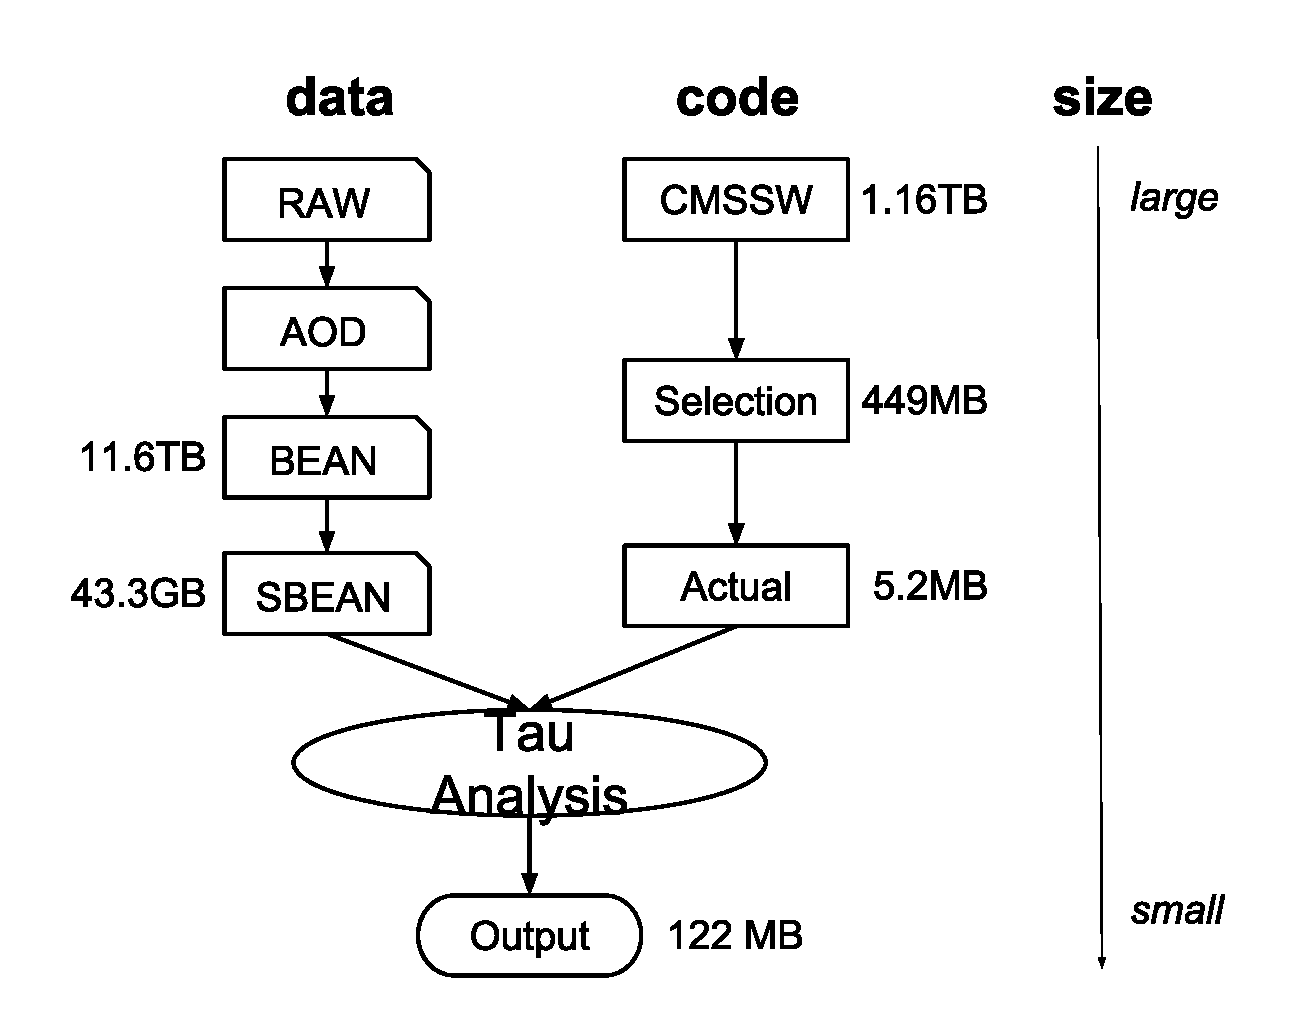
\includegraphics[width=.8\columnwidth]{data-code-size.eps}
\caption{Inputs to Tau Roast}
\label{fig:data-code-size}
\end{figure}

\begin{table}[t]
    \centering
    \small
    \begin{tabular}{|l|l|r|r|r|}
        \hline
        \bf Name & \bf Location & \bf Total & \bf Named & \bf Used \\ 
        \hline
        Ntuples data    & HDFS& 11.6TB & 43.3GB & 20GB \\ \hline
        CMSSW code     & CVS & 88.1GB & 448.3MB & 6.3MB\\ \hline
        Tau source       & Git & 73.7MB & 73.7MB & 73.7MB \\ \hline
        PyYAML binaries    & HTTP & 52MB & 51MB & 51MB \\ \hline
        .h file       & HTTP& 41KB & 41KB & 41KB \\ \hline
        Misc commands & PanFS & 155TB & N/A  & 1.6MB \\ \hline
        Linux commands & localFS & 110GB &  N/A & 68.3MB \\ \hline     
        Configuration & CVMFS & 7.4GB & N/A & 103MB \\ \hline
        HOME dir& AFS &10.2GB & N/A & 34MB\\ \hline
        Total      &    & 180.1TB            & N/A & 21GB \\ \hline
    \end{tabular}
    \begin{tablenotes}
      \small
      \item The first column illustrates the total size of each data and software source; 
            the second column illustrates the size of the named files from each source;
            the third column illustrates the size of acutally used data from each source.
            N/A denotes it is hard to figure out the named size of implicit dependencies directly.        
    \end{tablenotes}
    \caption{Data and Code Used by Tau Roast}
    \label{table:size-original-real}
\end{table}

\section{Overview of Tau Analysis}

Within the ongoing investigation of the Higgs boson at the CMS
detector, part of the LHC at CERN ~\cite{collaboration2008cms}, the Higgs production in association
with two top quarks allows to measure the Higgs coupling strength to
top quarks.  As the Higgs boson is to short-lived to be detected
itself, it has to be reconstructed from its decay products.

The application which is the study of this paper is called \emph{TauRoast}
It searches for cases where the the Higgs boson decays to two tau leptons.
The leptons are not observed directly, but by the particle showers
that they generate.  So, the analysis must search for detector
events that show a signature of decay products compatible with both hadronic tau and top decays.  Properties of such events are used to distinguish
the events of interest (Higgs decays) from all other events and
are also used in further statistical analysis.

Figure~\ref{fig:data-code-size} shows that both the code and data
that form \emph{TauRoast} are drawn from large repositories through
multiple steps of reduction.

{\bf Data Sources.}
The CMS collaboration provides analysis end-users with a pre-processed
and reduced data format, AOD ~\cite{holtman2001cms}, containing information for events, i.e.,
proton-proton collisions with a signature of interest, in the form of
reconstructed particles.  This format is based on the RAW output of
the CMS detector readout electronics and reconstructed world-wide.
Both real and simulated data are available for examination.

As AOD data are too large to be iteratively processed repetitively in
an physics analysis workflow, it is normally reduced further in
structural complexity and content.  For the analysis under
investigation here, this is a two-step process.  First, the AOD data
are processed at the Notre Dame working group cluster to BEAN events,
containing only trivial data containers packed in vectors.  This step
is time and CPU intensive and its output contains data of 11.6$\,$TB to be
analyzed by the tau analysis.
It is performed by a small custom code framework,
which is built on top of the CMS software stack, CMSSW ~\cite{cms2006cmssw},
and uses packages provided by several other special interest groups within CMS.
While the CMSSW framework is installed locally,
the various packages used are checked out from CVS,
and the BEAN framework is stored in git.
This is scheduled to change,
as the CMSSW distribution model switches to a virtual filesystem mounted via FUSE,
and special interest groups move their code to git.
The BEAN format, production code, and
data are shared within the analysis group looking at Higgs production
in association with top quarks, which is formed by groups from a few
American and European universities,
consisting of up to a few dozen contributors.

In the second step, which is the beginning of the actual tau analysis,
the data are reduced to variables relevant to the tau roast procedure, while
only events matching basic quality criteria are kept.  This results in
a dataset of 43.3$\,$GB.  Again, the Notre Dame CMS groups cluster
resources are used to perform this reduction and selection,
running highly customized software,
built on CMSSW and the BEAN framework,
but with output code written and maintained by a few people only.
Again, the code is stored in a git repository.

The final data analysis, investigated below, can be run as a single
process, and contains a stringent event selection to keep only high
quality candidate events for the underlying physical process (using
about 20$\,$MB of space).  Quantities from the selected events can be
both plotted and used in multivariate analysis to determine the level
of expected signal in real data.
This package is written using the CMSSW build framework,
but only utilizes code from ROOT,
a particle physics toolkit underlying CMSSW,
and a few external python dependencies for convenience.
The latter have to be manually fetched and installed,
while the analysis program is built by CMSSW after being checked out of git.

{\bf Code Sources.} Like many scientific codes, the central algorithm
of \emph{TauRoast} is expressed in a relatively small amount of
custom code developed by the primary author.  But, the code cannot
run at all without making use of an enormous collection of software
dependencies.  Some of these dependencies are standard to operating
systems worldwide, some are standardized across the entire high-energy
physics field, some are particular to small collaborative groups,
and a few are very specific to a single researcher.

The largest of these repositories is the CMS Software Distribution (CMSSW),
a carefully-curated selection of software packages which is distributed
in several forms.  Historically, components of CMSSW were obtained by checking components
of the source out of CVS, or by installing a complete binary package on a shared
filesystem within an HPC center.  In recent years, distribution has moved to
an on-demand delivery system known as CVMFS~\cite{blomer2011cernvm}.  The content
of CMSSW is managed very carefully by a centralized team whose main goal
is to ensure that the current version of the software operates correctly
on the operating systems and architectures currently in use.  However,
preservation is not an objective of the group, and so there is
no guarantee that old versions of CMSSW operate in new environments,
or vice versa. 

\section{Observations}

\emph{TauRoast} was provided to us in the form of an
email which described, in prose, how to obtain the source,
build the program, and run it correctly on one specific
machine at our home institution, with no particular guarantee that
it will run anywhere else in the world.
Although this starting point may seem extreme, it is
perfectly natural for collaborators to share configurations
with each other in this form, and to rely on the presence
of a working environment with appropriate dependencies already
installed.  From this starting point, the authors played the
role of curators, whose job it is to prepare the application
for permanent archival.

First, we elaborated the email instructions into an
executable script that obtains the dependencies and then
executes the analysis.  The script declares the necessary
environment variables, downloads and checks out the necessary source code,
builds it appropriately, calls initialization scripts in
the dependent software, and then runs the analysis.
A few rounds of correction with the original author were necessary
to obtain all the dependencies and run the artifact correctly.
(The original email also indicated how to run the application
within a production batch system.  For the purposes of preservation,
we consider the execution infrastructure to be distinct from the application,
and leave it out of consideration for now.)

The process of elaborating the program into a script revealed
several observations about this type of application:

\begin{itemize}

\item {\bf Many Explicit External Dependencies.}  TauRoast depends on a large number of
external dependencies, each with a different access method and data source.
While we knew in advance that it depended upon the large CMSSW distribution,
it was not apparent until elaborating the script that it depended upon
two different Github repositories for the Tau source,
a CVS server at CERN for some configuration information, a public web page
for the PyYAML library, and the public home page of a Notre Dame student
for one missing header file.  (The latter is particularly troubling!)
While, at some level, the authors and users of these software know of these dependencies, they are often missing in
informal communications or forgotten once the dependency is install.
However, once known, they are at least expressed explicitly within the script.

\item {\bf Many Implicit Local Dependencies.} A much harder problem is that the
application assumed the presence of many different components in the local
filesystem view.  It would be tempting to capture all of these by simply
storing a virtual machine image containing the local filesystem.  However,
the application dependend on no less than {\bf six} networked filesystems
available on a particular machine available to the author:
the data to be analyzed was stored on an HDFS~\cite{hadoop} cluster,
some configuration data was stored on a CVMFS~\cite{cvmfs} filesystem,
and a variety of software tools were on an NFS~\cite{howard1988scale},
pNFS~\cite{welch2008scalable} and AFS~\cite{sandberg1985design} systems.
The original authors were not aware of many of these dependencies,
because they simply relied on local administrators to configure the
software and make it available.

\item {\bf Configuration Complexity.}  As a means of controlling the complexity
of dependent software packages, the high energy physics community has developed
a number of tools that perform run-time configuration and consistency checks
of the available software.  {\tt scram} is the software management tool used
by the CMS experiment.  Before running any code, {\tt scram} is used to locate
the appropriate version software,  set environment variables such as the PATH, run any
tool-specific configuration, and do the same for all software on which it depends.
If the correct versions are not available, {\tt scram} halts and emits an error.
While this procedure has great value for consistency, it also introduces a significant cost
because it involves a large number of nested scripts traversing a filesystem,
repeatedly looking up metadata.  In our example, the time to perform this configuration
with a cold cache is about 14 minutes, which is almost as large as the actual analysis
run, which takes 20 minutes.

\begin{figure*}[t]
\centering
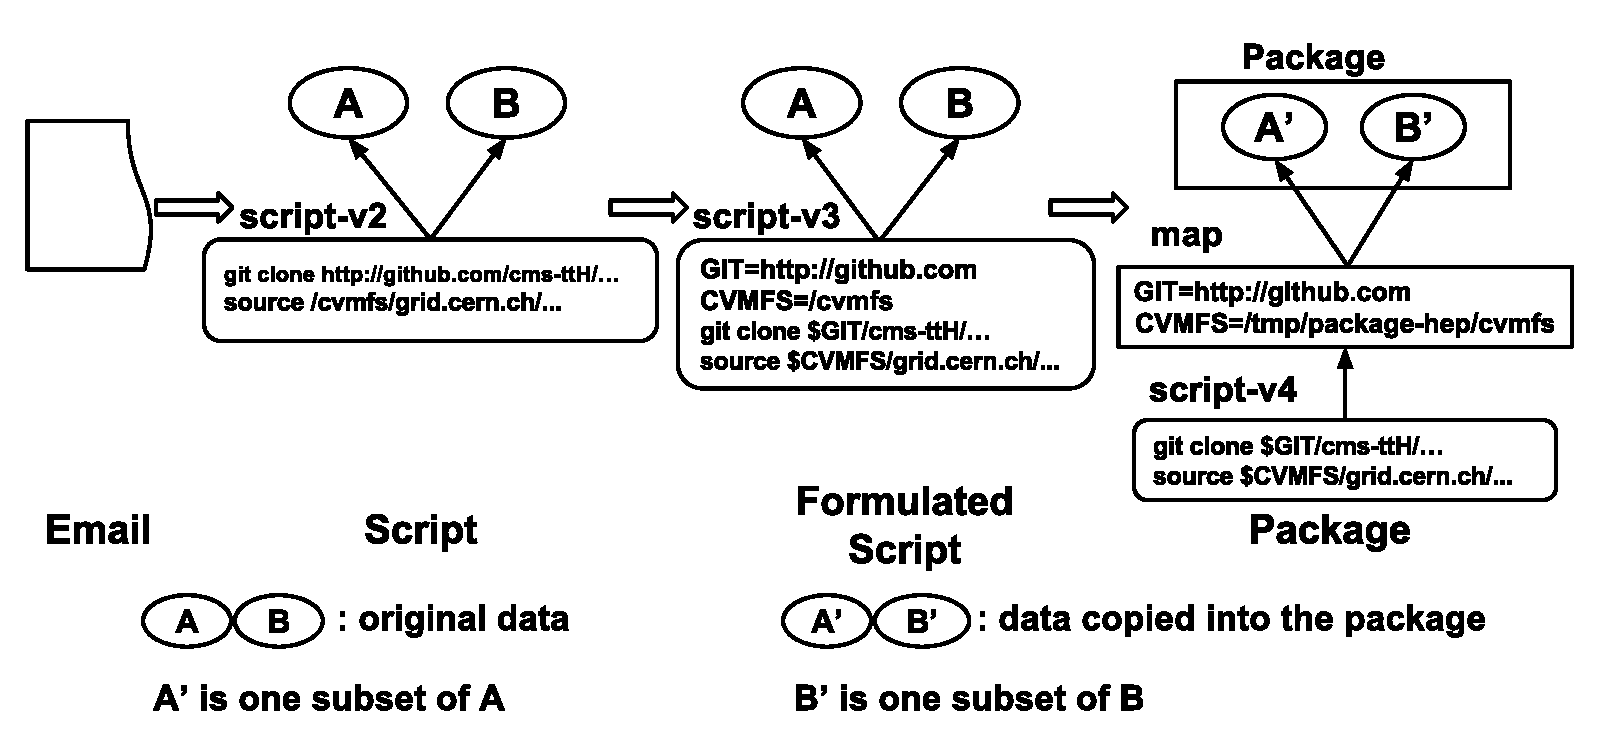
\includegraphics[width=1.6\columnwidth]{version-evolution.eps}
\caption{Version Evolution}
\label{fig:version-evolution}
\end{figure*}

\item {\bf High Selectivity.}  Although the total size of the resources accessed by this
program is very large, the size of the data and software actually used are much smaller.
Often, an entire repository or data source is named within the script, but the program
only needs a handful of items from that source.  For example, the data is stored on an
HDFS filesystem with 24TB of data, but only 43GB of that are the input Ntuples,
and of those only 20GB are actually consumed by the program. The CMSSW repository is 88GB in total
but only 448MB in source are checked out, and the software actually used only
measured 6.3MB.  In a few cases, a source of software is named but never actually accessed.
(For example, our original script includes the Open Science Grid software stack in the PATH, but does not actually use it.)
We suspect that end users are accustomed to missing dependencies and thus get in the habit of adding commonly used software,
whether it is needed or not.

\item {\bf Rapid Changes in Dependencies.}  Over the course of three months
between collecting the initial email, analyzing the program, and writing this
paper, the computing environment was under continuous change.  The CMSSW software
distribution released a new version, the target execution environment was upgraded
to a new operating system, and the experiment deprecated the use of CVS for obtaining
the software.  While the users of this software seem be accustomed to constant change,
any preservation technique will have to be very cautious about relying upon an
external service, even one that may appear to be highly stable.

\end{itemize}

\if 0

\begin{table}
    \centering
    \begin{tabular}{|l|}
        \hline
        {\bf Version 1: Email}\\ \hline
        1. Create a CMS release,\\
            \hspace{9pt} e.g. {\tt cmsrel CMSSW\_5\_3\_11\_patch3} \\
        2. Install the BEAN packages as the instructions: \\
            \hspace{9pt} {\tt \url{https://github.com/cms-ttH/BEAN/blob/...}}\\
        3. Install grid-control: \\ 
            \hspace{9pt} {\tt svn co \url{https://ekptrac.physik.uni-ka/...}} \\
        4. INstall the TauAnalysis package: \\
           \hspace{9pt} {\tt git clone \url{https://github.com/matz-e/...}} \\
           \hspace{9pt} {\tt scram b -j32} \\
        5. Fix grid\_control.cfg and run it. \\
        6. Perform the actual tau roast program. \\ 
        \hline
        {\bf Version 2: Script}\\ \hline
        {\tt setenv CMSSW\_BASE CMSSW\_5\_3\_11\_patch3} \\
        {\tt cmsrel \$HOME/\$CMSSW\_BASE} \\
        {\tt cvs co -r V03-09-23 PhysicsTools/PatUtils} \\
        {\tt git clone \url{https://github.com/cms-ttH/BEAN.git}} \\
        {\tt wget -r \url{http://nd.edu/~abrinke1/...}} \\
        {\tt scram b -j32} \\
        {\tt wget \url{http://pyyaml.org/download/pyyaml/PyYAML...}}\\
        \#the experiment data is from HDFS \\
        {\tt cd \$HOME/\$CMSSW\_BASE/src/PyYAML-3.10}\\
        {\tt cmsenv}\\
        {\tt python setup.py install --user} \\
        {\tt scripts/roaster data/generic\_ttl.yaml} \\ 
        \hline
        {\bf version 3: Formulated Script} \\ \hline
        {\tt setenv CMSSW\_BASE CMSSW\_5\_3\_11\_patch3} \\
        {\tt setenv {\bf GIT} \url{https://github.com}} \\
        {\tt setenv {\bf PYYAML} \url{http://pyyaml.org}} \\
        {\tt setenv {\bf ND} \url{http://nd.edu}} \\
        {\tt cmsrel \$HOME/\$CMSSW\_BASE} \\
        {\tt cvs co -r V03-09-23 PhysicsTools/PatUtils} \\
        {\tt git clone \${\bf GIT}/cms-ttH/BEAN.git} \\
        {\tt wget -r \${\bf ND}\url{/~abrinke1/ElectronEffectiveArea.h}} \\
        {\tt scram b -j32} \\
        {\tt wget \${\bf PYYAML}/download/pyyaml/PyYAML...}\\
        \#the experiment data is from HDFS \\
        {\tt cd \$HOME/\$CMSSW\_BASE/src/PyYAML-3.10}\\
        {\tt cmsenv}\\
        {\tt python setup.py install --user} \\
        {\tt scripts/roaster data/generic\_ttl.yaml} \\ 
        \hline
       {\bf Version 4: Fine-Grained Toolkit - Package}\\ \hline
        {\tt setenv CMSSW\_BASE CMSSW\_5\_3\_11\_patch3} \\
        {\tt setenv {\bf GIT} \url{https://github.com}} \\
        {\tt setenv {\bf PYYAML} \url{http://pyyaml.org}} \\
        {\tt setenv {\bf ND} \url{http://nd.edu}} \\
        {\tt cmsrel \$HOME/\$CMSSW\_BASE} \\
        {\tt cvs co -r V03-09-23 PhysicsTools/PatUtils} \\
        {\tt git clone \${\bf GIT}/cms-ttH/BEAN.git} \\
        {\tt wget -r \${\bf ND}\url{/~abrinke1/ElectronEffectiveArea.h}} \\
        {\tt scram b -j32} \\
        {\tt wget \${\bf PYYAML}/download/pyyaml/PyYAML...}\\
        \#the experiment data is from HDFS \\
        {\tt cd \$HOME/\$CMSSW\_BASE/src/PyYAML-3.10}\\
        {\tt cmsenv}\\
        {\tt python setup.py install --user} \\
        {\tt scripts/roaster data/generic\_ttl.yaml} \\ 
        \hline
    \end{tabular}
    \caption{Scripts of each Solution}
    \label{table:scripts}
\end{table}

\fi

\section{Preservation Strategies}

Figure~\ref{fig:version-evolution} illustrates the evolution history of
different preservation strategies. First, an email depicting how to repeat the
experiment is used. Then, all the necessary steps to reproduce the experiment
mentioned in the mail are collected into one shell script. In order to decouple
data sources and data references, one formulated script is introduced
to express all the dependencies at the beginning of the script in the form of
environment variables. Finally, this decoupling idea is further extended into
one map file which keeps the relationship between the data reference in the
script and the actual storage location. One independent package containing all
the data and software dependencies is generated to make the reproduction
process more easier.  

\subsection{Solution 1: Email}

In order to repeat Matthais's example, we consulted the original
author by email about the necessary work for the experiment. In response,
the original author introduced the general workflow of his tau roast program through one long
email including notes, linux shell commands, web linksi, as illustrated by the Version 1 of
Table~\ref{table:scripts}.

However, this solution to repeat one experiment has three potential drawbacks.
Firstly, the experience of repeating one tau roast program through emails is
chaotic. You need to constantly jump around multiple web links. There are overlap
between the content of the email and the content of web links, which needs the
new user to merge them. Multiple communication through emails is necessary to
ensure the successful reproduction of the whole analysis. For example, the original
email refers to one environment variable called CMSSW\_base without clear
declaration, the new user needs to send one email to the original writer to
obtain its accurate value. Secondly, the necessary procedures to repeat the
experiment, including software acquisition from different sources, is complex
for the new user. In the example, the sources of software includes
CMSSW, Git, HTTP. The access of CMSSW requires the new user to be an authorized
user of CMSSW. What's more, some parts of the workflow are unrepeatable. The
third step of this experiment requires the new user to own the access authority
of the Grid and involves the analysis of AOD data with the size of about 400TB.

Implication: Directly repeating the experiment using the workflow description and results provided by the original author is complex and difficult. Some extra work must be done to make the reproduction process easier.

\subsection{Solution 2: Script} One possible solution for the access authority
problem of Grid data is to grant the new user the authority to access gird data
directly. Another possible solution is let the new user directly operate on the
machine the original author used. As for the complexity of jumping between
multiple web links, people may suggest that the original author
should generate one script including all the contents from different web links.

To test out these possible solutions, we integrate the content of all the notes, commands and web links involved in the emails into one neat, complete shell script, which begins with the definition of environment variables, software acquisition from CMSSW, Git and other web resources, and software installation, ends with the execution of the actual analysis program. Version 2 of Table~\ref{table:scripts} illstrates the merged script. As for the data acquisition from the Grid, we directly use the local copy in HDFS to avoid requiring the new user to obtain a Grid certification.


%*****hmeng-doult: the size of hadoop need to reconsidered. how to correctly illustrate the data size of this example?

Because the script includes all the necessary procedures for the reproduction
of one analysis program, the readability and friendliness of this solution is
higher than that of the email format. 


\subsection{Solution 3: Formulated Script}
%%

The script can reduce the complexity of repeating one experiment through the integration of all the necessary procedures. However, the data and software dependencies are still randomly distributed across the whole script, which requires one complete scan of the script to obtain the  dependency list. 

To decouple data sources and data references and make the data dependencies clear, Version 2 of Table~\ref{table:scripts} is formulated into one new version, as shown in
the Version 3 of Table~\ref{table:scripts}. Each new environment variable at the beginning part of
the script is corresponding to one dependency. All the following access to data
or software dependency will refer to its corresponding environment variable.
All the environment variables of dependencies form one map, which maintains the
target address of each dependency.

This script style may function as one new guideline to the original author of
one experiment, which expresses the dependencies more clearly and expedites the
preparation process to repeat one experiment. The introduction of the map file
also reduces the workload of changing one dependency. For example, if we want
to utilize one new git package to analyze the same dataset, only the modification of
environment variable corresponding to the original git package is necessary.
Without the map mechanism, the whole script needs to be scanned to figure out and
replace all the references of the original git package.

So far, the data access authority is ignored and
the reproduction of the experiment is on the machine the original author used. 
As for Grid data, using the data
copy stored in the machine where the original author executed the experiment requires the
new user to have the authority to access the machine, which complicates the
management of the original machine, even is impossible if the original machine
executes rigid user access control. Granting everyone who wants to repeat the
analysis the access authority for Grid is unacceptable to system administrator. 

Implication: All the data and software involved in the experiment should be
provided to the new user in the format of one self-contained package so that
the new user can avoid 
access authority problems.
In addition, the requirements of the underlying
OS and hardware should also be figured out and provided to the new user.

\subsection{Solution 4: Fine-Grained Toolkit - Package}
The difficulty of data access authority acquisition enforces us to find out one
solution, in which the reproduction of the original analysis can be done
without any external dependency. That is, one independent and self-contained
package containing all the data and software dependencies is necessary. 

Someone may suggest that it should be the responsibility of the original author
to generate the required package. However, letting the original author provide
the package. 
One reason is that figuring out the underlying dependencies of
each software is complex and time-consuming and even impossible for the
original author. In this experiment, the machine used for the experiment is one
public machine of physics department, and the original author is one common user without
root authority. The underlying OS and supporting softwares are installed and
maintained by the IT department of the university. On the other hand, the
architecture design of the required package including all the data and software
dependencies is not under the research field of physists.

To generate one self-contained and independent package for one experiment, all
the clear and implicit dependencies must be figured out firstly. The map mechanism
of Solution 3 can provide clear data and software dependencies. As for the
implicit dependencies, directly preserving the whole OS together with the data
stored on the disk of the original machine or the data from other filesystems
mounted as local filesystems, such as HDFS and PanFS, is not feasible. One
efficient mechanism which can figure out the really used parts of all these
filesystems is necessary. The requirements of the underlying OS and hardware
architecture can be easily found with system tools such as uname or
lsb\_release.

Then one new package including all the data and software dependencies can be generated and published. 
One packaging utility is necessary for the original author to generate the package. 
To multiplex the common data which is involved in different experiments, such as OS images and common software libraries, the data of different packages will be rearranged and categorized in the archive.
One description file, which includes the experiment aim, dependency list,  package size and relevant information, will be generated for each package.

\begin{figure}
\centering
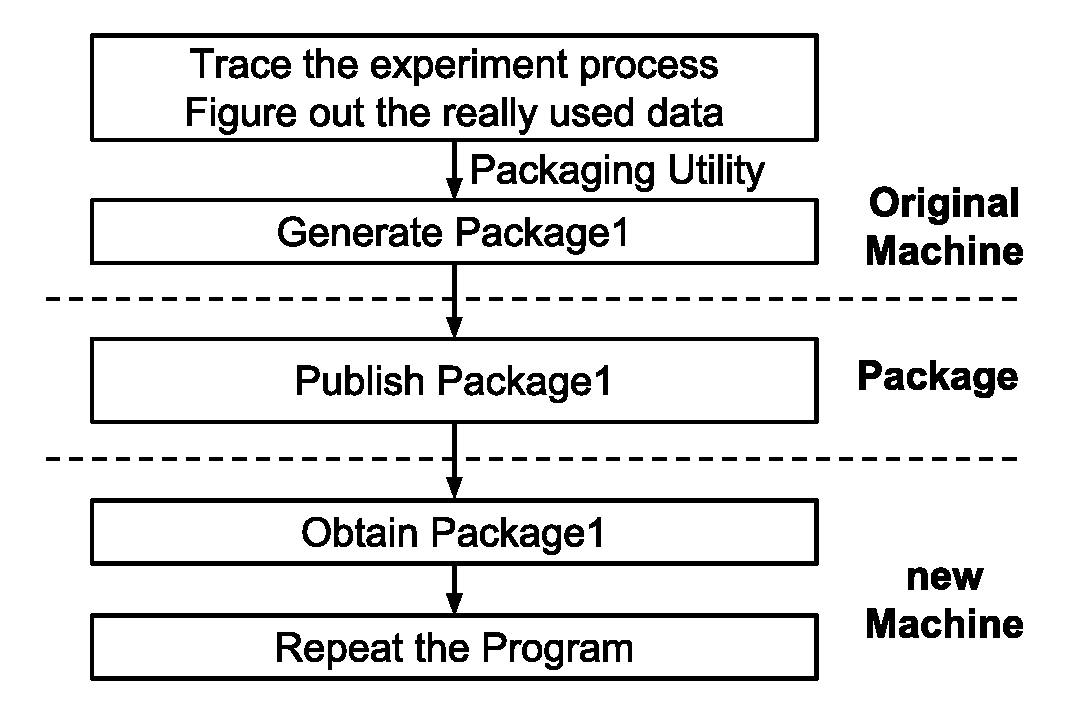
\includegraphics[width=.8\columnwidth]{solution3.eps}
\caption{Relationship of Roles}
\label{fig:solution3}
\end{figure}

The relationship of different roles involved in the experiment preservation and
reproduction is shown in Figure~\ref{fig:solution3}.  The original author is
responsible for generating one package with the help of the packaging utility. Then the package, together with
its map file and description file will be uploaded into the archive. When
another scholar wants to repeat the experiment, one copy of the package and its
corresponding map file will be downloaded into the new machine.

\begin{table}
    \centering
    \begin{tabular}{|l|l|}
        \hline
        \bf Archive Path & \bf Service Description \\ \hline
        {\tt /archive/OS/path} & OS Image \\ \hline
        {\tt /archive/software/path} & Common Software Library \\ \hline
        {\tt /archive/CMSSW/path} & CMS Software Library \\ \hline
        {\tt /archive/git/path} & Git Software Library \\ \hline
        {\tt /archive/http/path} & HTTP resources \\ \hline
        {\tt /archive/experiment/path} & experiment private files \\ \hline
        {\tt /archive/grid-data/path} & data from the Grid \\ \hline
    \end{tabular}
    \caption{Structure Organization of the Archive}
    \label{table:archive-map}
\end{table}

Table~\ref{table:archive-map} illustrates the structure of the remote archive.
Item {\tt /archive/OS} includes the images of different Operating Systems.
Item {\tt /archive/software} integrates all the commonly used software, such as git,
python, perl. The archive also organizes the data from CMSSW, Git, HTTP and the
Grid. Item {\tt /archive/experiment} includes the all the experiments submitted into the
archive. The private files and description files of each experiment will be
organized together.

The Version 4 of Table~\ref{table:scripts} illustrates the script used in
Solution 4, which is the same as the one used in Solution 3. 
However, one map file is necessary for the relocation of the data access targets, as
show in Figure~\ref{fig:version-evolution}. 
The map file redirects the git access path into {\tt /archive/git} from the original path (\path{http://github.com}) referred in the script.
This design decouples the experiment script and the actual data access targets, which minimizes the impact of the evolution of different data dependencies
and ensures the transparent access.
The modification of the archive only introduces the minimal changes of the map file on the client side.

The archive supports two different data preservation models: Internal and External. Internal method will preserve the data in the archive. External method refuses to preserve the content of data, but only preserve the reference to the actual storage place of data. For example, the size of experiment data from the Grid is extremely large, and storing the same data in the archive is time-consuming and space-consuming. Through External method, the archive only preserves one reference to the data inside the remote Grid.

This solution tries to create one self-contained and independent package for
each experiment and integrate different packages for different experiments into
one archive to multiplex common data. One packaging utility, which can figure out all the really used data of one program  will be provided
to help the original author to generate the package. The archive can maintain
the experiment dependencies through Internal or External method. The archive
itself will be responsible for the data maintenance and relevant authority
access problem. The new user can repeat one experiment through the
interaction with the archive.

\section{One Implemention of Fine-Grained Toolkit Using Parrot}

The section introduces our implementation of one fine-grained packaging utility based on Solution 4. With the help of one
virtual filesystem access tool, Parrot ~\cite{thain2005parrot}, we trap all system calls of one
program through ptrace debugging interface, and collect all the names of accessed files. 
Then one self-contained package containing all the accessed files is generated to help others repeat the experiment.

\subsection{Working principle of Packaging Utility} 

Parrot is a virtual filesystem access tool which attaching existing programs to
a variety of remote {\tt I/O} systems including 
HTTP, FTP, GridFTP, iRODS, HDFS, XRootD, GROW, and Chirp. It traps all system calls of one program through ptrace
debugging interface, and replaces them with remote {\tt I/O} operations as desired.
Through executing one program under Parrot, all the paths of files involved in
this program can be recorded.  

With the help of Parrot, one packaging utility which generates one independent
package for one program to make the reproduction of the program convenient can
be deployed. The starting point of the packaging utility is one successful execution
sandbox (the data from Grid has been preserved in HDFS and the software from
CMSSW, Git and HTTP has been on the local machine.). We re-execute the actual
data analysis code under Parrot and get the name list of all the files actually
accessed during the execution process of the actual data analysis. Then,
according to the filename list, one package containing all the necessary data
and software for one analysis program is generated. Next time, when another
scholar wants to repeat the program, he only needs to obtain the package and
directly execute the actual analysis program inside the package. 
Figure~\ref{fig:solution3} illustrates the working principle of the packaging utility.

\begin{table}
    \centering
    \begin{tabular}{|l|}
        \hline
        {\tt set CMSSW\_BASE = (CMSSW\_5\_3\_11\_patch3)} \\
        {\tt cd \$HOME/\$CMSSW\_BASE/src/PyYAML-3.10}\\
        {\tt cmsenv} \\
        {\tt python setup.py install --user} \\
        {\tt cd \$HOME/\$CMSSW\_BASE/src/ttH/TauRoast}\\
        {\tt scripts/roaster data/generic\_ttl.yaml} \\
        \hline
    \end{tabular}
    \caption{Script of Fine-Grained Toolkit using Parrot}
    \label{table:parrot-script}
\end{table}

Table~\ref{table:parrot-script} illustrates
the simplified script, which
only contains the necessary environment variables and the
actual analysis command.

\subsection{Workflow of Packaging Utility}
\begin{figure*}
\centering
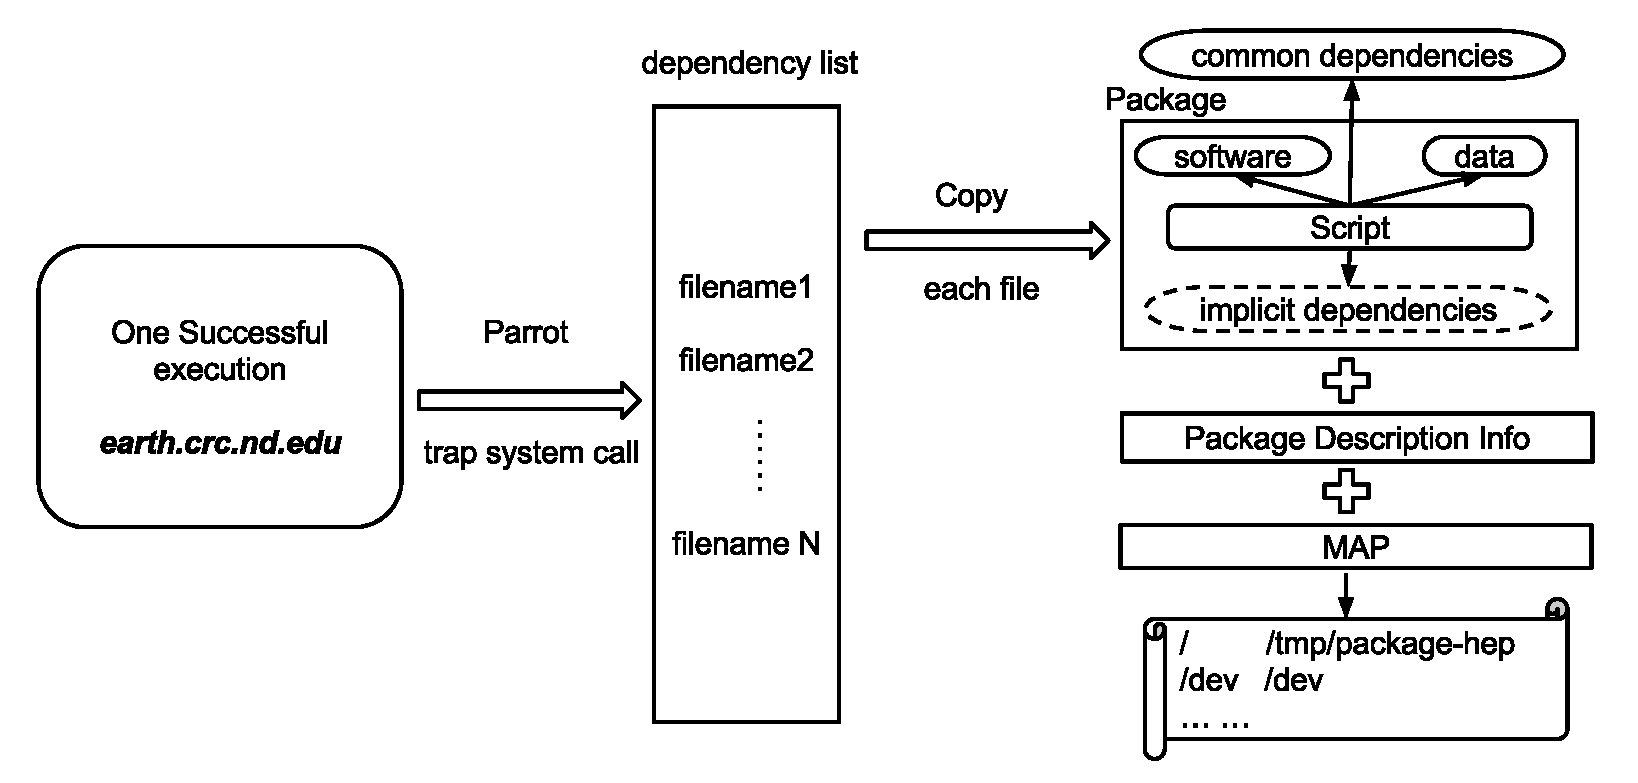
\includegraphics[width=1.6\columnwidth]{workflow-parrot.eps}
\caption{Workflow of Solution 4}
\label{fig:workflow-parrot}
\end{figure*}

Figure~\ref{fig:workflow-parrot} illustrates the workflow of this solution. Firstly, execute the analysis program under Parrot and obtain one filename list containing all the accessed files. Then generate one package containing all the files included in the filename list. Finally, rerun the program with the help of the package. Each step will be examined in details.

{\bf(1)} Execute one analysis program under Parrot and obtain filename list (L1) of it

Parrot is one virtual file system that can support user access to multiple
underlying file systems. Parrot traps each system call involved in the process
of data access, figures out the type of file system and redirects it into
corresponding operations to the accessed file system. During this process, each
accessed file, together with the access type, such as
open, stat, read and write, is recorded into one file.

The command used to generate the filename list is as follows. The {\tt name-list} parameter refers to the path of the file containing all the accessed file name of the experiment.

{\tt parrot\_run \texttt{-{}-}name-list namelist /bin/tcsh script\_v4.sh}

The original ouput of this command is one namelist file with the size of 6.6MB
and 132,047 lines, each of which corresponds to one one accessed file of the
program. We noticed that some items appeared multiple times in the filename list. To reduce the
packaging time, de-duplication and sorting techoniques are used for the
namelist file, generating one smaller file with the size of 3.2MB and 67,168 lines.

{\bf (2)} Generate one package containing the files of L1 

The packaging utility iterates each filename inside L1 and copies it into the
target package. Finally, the target package
together with its description information, and one map file, which redirects
the access of files from different file systems into the files inside the target package, will be
generated as the output of this step. The packaging process also runs within Parrot environment to
access data from different file systems.

The command used to generate the package is as follows. 
{\tt package-utility.sh} is a bash script which iterates each line of L1 and
determines the behavior according to the file type (common files, directories,
symbolic link files) and the system call type.
The package description information is shown in Table~\ref{table:package-info}.

\begin{table}
    \centering
    \begin{tabular}{|l|}
    \hline
     the total size of package: 21GB \\ 
    the total number of files: 15905\\ 
    the total number of directory: 1549\\ 
    the total number of symbolic link: 4614 \\ \hline 
    \end{tabular}
    \caption{Package Infomation}
    \label{table:package-info}
\end{table}

{\tt parrot\_run /bin/bash package-utility.sh -L namelist}

%*****lack: file content + metadata; only file metadata; different process
%solutions
Each file inside L1 except for common dependencies is copied into the package, the final path of the file
becomes the path of the package, followed by the original file path. In this
program, the path of the package is {\tt /tmp/package-hep}, so the final path of one
file with the original path path1 is {\tt /tmp/package-hep/path1}.

The map relationship between the file access path used in the actual analysis
program and the actual file location used during the reproduction process is
kept inside the map file, as illustrated in Table~\ref{table:map-file}.

To ensure the successful reproduction, the filesystem structure of the original
execution environment should be preserved as completely as possible. However,
attempting to copy the whole content of one directory or one file is
space-consuming and time-consuming, because the original program may only
access the metadata of one file with the size of 200GB. Our solution is to
determine the copy degree of one directory or one common file according to the
type of the system call.


\begin{table}
    \centering
    \begin{tabular}{|l|l|}
    \hline
    \bf Path used in Program & \bf Actual Location \\ \hline
    {\tt /} & {\tt /tmp/package-hep} \\ \hline
    {\tt /tmp/package-hep} & {\tt /tmp/package-hep} \\ \hline
    {\tt /dev} & {\tt /dev} \\ \hline
    {\tt ...} & {\tt ...}\\ \hline
    \end{tabular}
    \caption{Structure of Map File}
    \label{table:map-file}
\end{table}

%*****lack: re-execute process: re-execution process will redirect all the data access into the package except for data under proc sys dev selinux
{\bf (3)} Repeat the analysis program using the package

When another scholar wants to repeat the analysis program, 
the description of the exepriment environment is firstly referred to build the underlying OS and basic software environment. In this example, the only necessary software basis is Parrot. Then the scholar can obtain one copy of the package and its map file, and rerun the program using the following command. The {\tt m} parameter can be used to refer to the path of map file, which will be explained in the next part.

{\tt parrot\_run -m /tmp/mountlist /bin/tcsh script\_v4.sh}

\subsection{Structure of Map File} 

The map file of one package supports pattern matching semantics,
which greatly reduces the scale of the map file and improves the efficiency of file path redirection. 
For example,
one item inside the map file is {\tt /dir1 /package-dir1} means that the access to each file and
subdirectory under {\tt /dir1} will be redirected into {\tt /package-dir1}.
If the semantics of the map file do not support pattern matching, the size of the map file will become astonishing. 
{\tt /dir1} may contain thousands of files, which will generate thousands of map items and take more time to redirect file paths.

During the packaging process, we notice
that it is impossible to copy the files under certain directories.
For example, during namelist acquisition process, three special files under {\tt /dev} directory were recorded into the namelist: tty, null and urandom, which are used for input and output.
Trying to copy these files into the new package would cause the packaging utility halt.
We also notice that copying the files under directories like {\tt /proc} is
meaningless. Because the process id of one program is random and depends on the
current allocation of process ID. 

As for these special file paths, letting
the program directly utilize the files on the new machine, where the new user
repeats the program, is a better choice. The semantics is implemented by
setting the target path of one file equal to the origin file path inside the
map file. For example, {\tt /dev /dev} means that when the program needs to access
files under {\tt /dev} directory, it will directly use the file under {\tt /dev} on the new machine, which is
independent from the namespace of the package. This semantics also make the
reference of files outside the package possible. If the new user wants to
expand the analysis of one program to his own data with the path of {\tt /A}, he can add the analysis
code into the analysis script and add one item {\tt /A /A} into the map file.


\subsection{Discussion of Solution 4} 

Under Solution 4, the reproduction of one analysis program becomes easier.
Rethink the example, the reproduction only needs
to set necessary environment variables, the actual analysis command
and the package. If different scholars want to repeat one analysis program,
what they need to do is to obtain the package and rerun the actual analysis
program. Under Solution 2, each scholar needs to get the necessary data and
software, and then prepare software environment. 

%here is the new content-hmeng
The starting point of Solution 4 is one successful execution on the original machine. 
Parrot traps all the system calls and copies each accessed file (except for common dependencies) into one package.
The necessary scientific data and software dependencies will be copied into the target package.
Strictly speaking, the concept of software and the concept of the scientific data are lost in Solution 4, because
the granularity of parrot is file.
The same thing happens to networked resources.
Packaging utlity maintains one list of common dependencies and first judges whether the file belongs to this list before trying to copy one file into the package.
%the following subsection belongs to the "discussion of data and software
%preservation" section

\begin{table*}
    \centering
    \begin{tabular}{|l|r|r|r|}
        \hline
        \bf Solution ID & \bf Data Resources &\bf Software Resources & \bf Operation Manual \\ \hline
        Solution 1& Grid & CMSSW Git HTTP & email \\ \hline
        Solution 2 and 3& local (HDFS) & CMSSW Git HTTP & shell script \\ \hline
        Solution 4& package & package & user manual of package \\ \hline
    \end{tabular}
    \caption{Relationship of Different Solutions}
    \label{table:relationship}
\end{table*}

%The fourth solution should be based on the third solution. during the packaging process, packaging utility first checks whether the file has been inside the target package, (if exists, whether it is the latest version). only if the file does not exist in the target package or the file in the target package is not the latest version, the packaging utility copies the file into the target package.

%*****hmeng-doubt: potential risk: different analysis programs share some common file names, but with different file contents. we should analyze the possibility of conflict: data.

%*****hmeng-doubt: in the fourth version, let user to mark whether they change the data and software. if changed, one new package is generated to avoid data overlap and pollution. otherwise, directly starts packaging process based on the current target package. 
\section{Evaluation}
The section first illustrates the relationship of different preservation and reproduction solutions, then the platform used to evaluate different solutions is introduced. The execution time and data size of Solution 2 and 4 are tested and compared. It is hard to accurately calculate the time consumption of Solution 1. Solution 3 shares the same time consumption and data size with Solution 3.

\subsection{Relationship of Different Solutions}
The relationship of these four solutions to repeat one program is shown in Table~\ref{table:relationship}. Each new solution tries to make it easier to repeat one program through making the data and software preparation easier.

\subsection{Evaluation Platform}

The first three solutions are all directly verified on the machine the original
author used to execute the experiment, which is convenient but involves access
authority problem. Solution 4 is verified on the original machine and on one virtual machine.
To compare the execution time and data size of Solution 4
with Solution 2, the package generated on the original machine is utilized to
rerun the experiment on the original machine. This choice avoids the impact of
different CPUs of the original machine and the new machine to repeat the
experiment. 

To completely verify the correctness of Solution 4, one virtual
machine ~\cite{goldberg1974survey} sharing the same kernel version with the original machine is deployed.
Then the necessary software environment is configured on the virtual machine,
and the package is copied onto it, and the
experiment is repeated on the virtual machine.

One virtual machine from amazon EC2 ~\cite{amazon2010amazon} is used to verify the reproducibility of the experiment. Table~\ref{table:config-vm} illustrates the configuration of the original machine and each virtual machine. 
All the machines adopt x86\_64 hardware platform and linux OS.
Both the local VM and EC2 VM repeat the experiment with the help of the package generated on the original machine successfully.

\begin{table}
    \centering
    \begin{tabular}{|l|r|r|r|r|}
    \hline
    \bf Machine & \bf Kernel Version & \bf Distro & \bf CPU & \bf Mem\\ 
    \bf Type &  & \bf Version & \bf Cores & (\bf GB)\\ \hline
    earth  & 2.6.18-371.4.1.el5 & RedHat 5.10 & 64 & 125 \\ \hline 
    local VM& 2.6.18-371.4.1.el5 & CentOS 5.10 & 4 & 2 \\ \hline
    EC2 VM& 2.6.18-348.el5xen & RedHat 5.9 & 16 & 60.5 \\ \hline
    \end{tabular}
    \caption{Configuration of Different Machines}
    \label{table:config-vm}
\end{table}



The configuration of earth machine. The configuration of our virtual machine. The configuration of amazon ec2.
each vm: data download time; untar time; script execution time;

\subsection{Evaluation of Solution 2}
The breakdown of execution time of Solution 2 is shown in Table~\ref{table:time-2nd}. About 40\%  of the total execution time is consumed to prepare relevant software environment. The cvs command is called to check out 23 packages from CMSSW and three git repositories are cloned.

\begin{table}
    \centering
    \begin{tabular}{|l|r|r|}
    \hline
    \bf Sub-Task & \bf Time & \bf Percentage \\ \hline
    Obtain software from CMSSW & 7min 24s & 21.44\% \\ \hline
    Obtain software from Git & 9s & 0.43\% \\ \hline
    Obtain software from Wget & 38s & 1.83\% \\ \hline
    Environment build - SCRAM & 5min 48s & 16.80\% \\ \hline
    Environment build - Python & 1s & 0.05\% \\ \hline
    Data analysis & 20min 31s & 59.44\% \\ \hline
    Total & 34min 31s & 100.00\% \\ \hline
    \end{tabular}
    \caption{Breakdown of Execution Time of Solution 2}
    \label{table:time-2nd}
\end{table}

This solution does not support mining of implicit dependencies.
The size of data and software from each category is shown in table~\ref{table:datasize-2nd}, which only lists the size of each clear dependency.

\begin{table}
    \centering
    \begin{tabular}{|l|r|}
    \hline
    \bf Data Category & \bf Data Size \\ \hline
    Software from CMSSW & 448.3MB \\ \hline
    Software from Git & 73.7MB \\ \hline
    Software from Wget & 52MB \\ \hline
    HDFS & 43.3GB \\ \hline
    Total & 43.86GB \\ \hline
    \end{tabular}
    \caption{Data Size of Solution 2}
    \label{table:datasize-2nd}
\end{table}

\subsection{Evaluation of Solution 4} 

The breakdown of execution time of the
Solution 4 is illustrated in Table~\ref{table:time-3rd}. The time used to
obtain filename list and generate P1 is greatly longer than the execution time
within the new package. However, the time consumption of filename list
acquisition and package generation is one-time. That is, once the package is
generated, many users can directly obtain the package and repeat the experiment
separately. 

\begin{table}
    \centering
    \begin{tabular}{|l|r|}
    \hline
    \bf Sub-Task &\bf Time \\ \hline
    Obtain file namelist & 28min 23s \\ \hline
    Generate P1 & 85min 51s \\ \hline
    Re-run the program within P1 & 13min 4s \\ \hline
    \end{tabular}
    \caption{Time Breakdown of Solution 4}
    \label{table:time-3rd}
\end{table}

The data size of Solution 4 is shown in Table~\ref{table:datasize-3rd}. The
data categories are more complex than our imagination. Except the data stored in
Hadoop and the necessary set of software, files from local filesystem and several remote filesystems, such as PanFS, CVMFS, NFS, and AFS, are also necessary for the reproduction of the program.

\begin{table}
    \centering
    \begin{tabular}{|l|l|r|}
    \hline
    \bf Data &\bf Location & \bf Data \\ 
    \bf Category & & \bf Size\\ \hline
    HDFS & hadoop &20GB \\ \hline
    PanFS & pscratch & 1.6MB \\ \hline
    CVMFS & cvmfs &103MB \\ \hline 
    NFS & opt &53KB \\ \hline
    AFS & afs &34MB \\ \hline
    Local FS& bin etc lib lib64 sbin tmp usr&68.3MB \\ \hline
    Total & &21GB \\ \hline
    \end{tabular}
    \caption{Data Size of Solution 4}
    \label{table:datasize-3rd}
\end{table}    

\subsection{ Data size Comparison of Solution 2 and 4}

The packaging utility checks the system call of each file within the namelist,
and maintains the minimum dataset, which makes the size of the final package 
as small as possible. The total size of Hadoop under Solution 2 is astonishing,
while the size of Hadoop under the package is decreased to 20GB. 
The total size of PanFS is 155TB, however, the size of the really used data of PanFS is only 1.6MB.
Table~\ref{table:datasize-2nd3rd} compares the original size and the really used size of each data source.
Solution 4 reduces the total size of all data sources from 156TB to 21GB.

\begin{table}
    \centering
    \begin{tabular}{|l|r|r|}
    \hline
    \bf Data Category & \bf Solution2: Size & \bf Solution4: Size \\ \hline
    HDFS & 43.3GB & 20GB \\ \hline
    PanFS & 155TB & 1.6MB \\ \hline
    CVMFS & 7.4GB &103MB \\ \hline
    NFS & 862GB &53KB \\ \hline
    AFS & 10.2GB &34MB \\ \hline
    Local FS& 110GB&68.3MB \\ \hline
    Total & 156TB &21GB \\ \hline
    \end{tabular}
    \caption{Data Size Comparison beweeen Solution 2 and 4}
    \label{table:datasize-2nd3rd}
\end{table}

\subsection{Execution Time Comparison of Solution 2 and 4}

Table~\ref{table:time-2nd3rd} shows the execution time comparison between
Solution 2 and 4. The time consumption of the reproduction of one program from
different scholars kept the same under Solution 2, including software and data
preparation. However, under Solution 4, the data and software preparation is
one-time. The following reproduction of the same program only needs to obtain
one copy of the package and execute the actual experimental analysis directly.
Data is obtained through accessing HDFS in Solution 2, but is copied into the package in Solution 4. This localization of experimental data speeds up the data analysis process, resulting the actual analysis time reducing from 20 minutes to 13 minutes.

\begin{table}
    \centering
    \begin{tabular}{|l|r|r|}
    \hline
    \bf Task & \bf Solution 2& \bf Solution 4\\ 
    \bf Category & \bf Time & \bf Time \\ \hline
    Software Acquisition & 8min 11s & N/A \\ \hline
    Environment Build & 5min 49s  & 3s \\ \hline
    Obtain file namelist & N/A & 28min 23s \\ \hline
    Generate package & N/A & 85min 51s \\ \hline
    Actual Analysis & 20min 31s & 13min 4s \\ \hline
    \end{tabular}
    \caption{Execution Time Comparison between Solution 2 and 4}
    \label{table:time-2nd3rd}
\end{table}    

\subsection{Excution Time on Different Machines}
Table~\ref{table:time-vm} shows the execution time of the experiment on different machines - the original machine, local VM and EC2 VM. 
Each machine utilizes the package generated on the original machine (i.e. earth) to repeat the experiment.
The execution time on one machine greatly depends on its hardware configuration, which is shown in Table~\ref{table:config-vm}.


\begin{table}
    \centering
    \begin{tabular}{|l|r|}
    \hline
    \bf Machine Type & \bf Execution Time \\ \hline
    earth & 13min 4s \\ \hline
    EC2 VM & 13min 30s\\ \hline
    local VM & 21min 38s \\ \hline
    \end{tabular}
    \caption{Execution Time on Different Machines}
    \label{table:time-vm}
\end{table}




%*****hmeng-doubt:Another reason for the packaging utility is that not all the data and software generated by the second version script is used during the the actual data analysis. The packaging utility can help us find out the optimal subset of data and software involved in one actual data analysis. 
%*****hmeng-doubt: this point is not the motivation. but one achievement comes together. out of imagination.
\section{Discussion of Data and Software Preservation}

This section concludes the important lessons of data and software preservation and experiment reproduction learnt from this case study. 
The necessity of preservation integration of multiple programs, preservation granularity, how to preserve large data, how to mine data and software dependencies,
the presrvation degree of the original filesystems, the importance of investigating user access model of data and software, will be discussed. 

\subsection{Preservation Integration of Multiple Programs}

Different experimenters may execute different analysis
programs on the same dataset using the same or overlapping sets of software.
Generating one new package for each analysis program from scratch is
time-consuming and space-consuming, which makes one data and software
preservation mechanism, that can integrate the preservation requirements of
different analysis programs, become necessary. 

\begin{figure}
\centering
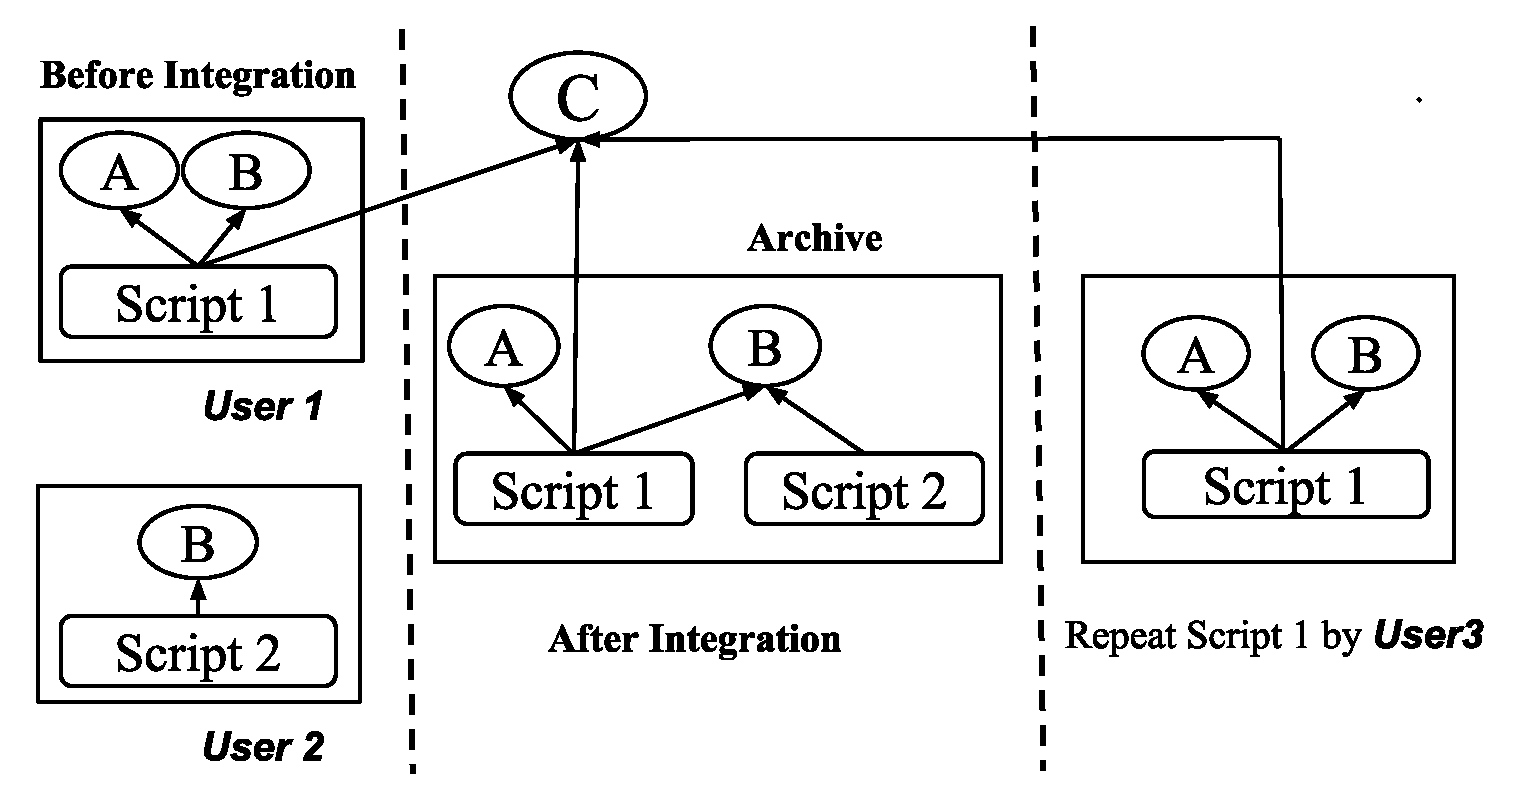
\includegraphics[width=1\columnwidth]{preservation-integration.eps}
\caption{Preservation Integration of Multiple Programs}
\label{fig:Preservation integration}
\end{figure}

To integrate the data and software from multiple analysis programs into one
archive, the concrete information of data and software, such as size, version,
source and the number of files, need to be recorded. 
The packaging
process needs to be re-organized. Packaging utility needs to maintain one list
of current software and data subset already stored in the archive. When one
user utilizes the packaging utility to preserve one program, the
packaging utility scans the script, gets the data and software dependency
part, judges whether each dependency has been inside the package, and only adds
the new data and software into the archive, and updates the package information
and relavant retrieval information.

The architecture of preservation integration of multiple programs is shown in
Figure~\ref{fig:Preservation integration}. Script 1 and Script 2, sharing one
dependency B, belongs two different programs. Without preservation
integration, B will be preserved twice in the archive. To improve the utilization efficiency of storage resources,
preservation integration of multiple programs is necessary. In the archive,
only one copy of B is stored, which is referred by both scripts.

\subsection{Preservation Granularity}

Another important factor of data and software preservation is the choice of
preservation granularity. In our implementation of Solution 4, the preservation granularity is one
file, because Parrot virtual filesystem traps each system call and redirects
the access path of each file. As a result, during the packaging process, each
time only one file can be copied into the target package, which is
low-efficient. However, there are other options of preservation granularity.
The software is generally preserved in the unit of package inside the remote
repository, the packaging process of one experiment can adopt one package as
the unit. In addition, if the size of one whole software repository is small
and the access frequency of each package inside it is high, the granularity can
be set to the whole repository.

\subsection{Preservation of Large Data}

The preservation policy must concern about the size of data. If data size is
small, copying it into one pacakge and transferring it between different
machines is not a bad idea. Howerver, when the size becomes large, copying it
into one package will make the size of the package uncontrollable. In
Figure~\ref{fig:Preservation integration}, the size of C is very large and
easily to be obtained through Internet by different users. Directly referring C
as networked resources is more efficient than preserving it into one package.

\subsection{Mining of Dependencies} 

The mining degree of data and software dependencies greatly determines the
repeatability of one experiment. Clear data dependencies is easy to figure
out, but how to figure out implicit data dependencies is complex. The situation
of software dependencies is more complex. The software dependencies include OS,
hardware platform, direct software dependencies and indirect software
dependencies.
The first
three categories are easy to deal with. The acquisition of indirect software
dependencies needs more efforts. 

One solution is to treat the computing environment, software environment
and scientific data as one integral entirety and preserve the entirety
completely. The reproduction of one experiment using this solution is easier.
However, the original machine is not only for one special experiment and may
concern a large amount of software and data unrelevant to the experiment. The
time and space overhead of this solution must be considered.

Another solution is to utlize package management
tools, like rpm, pacman, apt, to recursively trace each direct software
dependency and generate one clear dependency graph. With the dependency graph,
the new user can configure the software environment and repeat the experiment.

The third solution is to trace the system calls of the experiment execution process
and record the paths of accessed files, which including the files of software dependencies.
Parrot adopts this solution. Even if git is one software dependency, there is no necessary to install git on the new machine.
All the files to guarantee the accurate execution of git has been copied into the package.

%\subsection{The preservation} When the authors and the programs becomes more
%and more, the whole pool of one repo may be nearly to be preserved. why not
%directly copy the whole repo and preserve it at the begining directly?  Answer:
%we must concern the efficiency of repeating one small and simple program.
\subsection{Preservation Degree of Directory Structure}

Data and software preservation of physics experiments must concern the
preservation degree of the original filesystem.  The three core components of
one filesytem are file, directory and metadata.  The access of files can be
divided into two categories: only access file metadata, like size, ownership,
access authority list, and access both the file content and metadata.  If both
the content and metadata need to be accessed, the whole file must be copies
into the package.  However, if only the metadata of one file is accessed, how
to preserve the file needs to be considered carefully. If the file size
is 1KB or 1MB, preserving the content is acceptable. If the size of one file is
1GB, preserving the whole file just for accessing its metadata is
inefficient.  

Directory is one list of files and subdirectories under it. At first, we only
copy the accessed items under one directory and ignored the unaccessed items.
However, some operations on one directory depends on each item under it. For
example, {\tt ls /dirA} is one linux command to list the name of each item under
{\tt /dirA}. Because the directory itself has the name list of items under it, only
the path of the directory is recorded into the namelist in the first phrase of
Solution 4. However, when we repeat the command {\tt ls /dirA} using the preserved package, it returns NULL because none of items under it exists in
the package, the behavior of the whole program will become incorrect
and unpredictable. 

To ensure the semantics of the original program, all the items under one directory must be copied
into the package. However, the
time and space overhead appears again. Currently, Solution 4 creates one item
with the same name but the size of zero for each item under {\tt /dirA}. Another
solution is to introduce one database to preserve the metadata of each file and
directory. 

\subsection{User Access Model of Data and Software}

The user access module of remote data
and software has a great impact of the preservation mechanism, especially when
we try to integrate the preservation of multiple programs. If all the programs
only refer the original data and software and refuse to modify them, the
preservation is easy and can ignore the data version problem. However, if some
programs try to modify the original data and software to accustom to its own
requirement, the preservation mechanism must provide one way to differentiate
the original data and the special data used in one certain
program. To have a clear understanding of the data access model, more examples
need to be investigated.

\subsection{Here is the Useful Package}

At the beginnig of our case study, we generated one package for the
example based on Solution 4. Several months later, the original machine met
some problems and the access model of CMSSW was also modified. In this case, if
you want to repeat the example on the original machine, different 
configurations, including CMSSW\_ARCH, environment variables and CVS access
authority need to be modified. However, with the generated package and its map file, we can repeat the experiment directly on the same machine without any modification.
%here is the new content-hmeng

\section{Related Work }

Generally, there are three approaches to preserve software environment:
hardware preservation, migration and emulation.  Hardware
preservation preserves the original software and its original operating
environment. 
Software migration technique \cite{cifuentes1996binary,mancl2001refactoring} was used to facilitate running software on new machines.
However, migration often involves the re-compiling and re-configuring
the source code to accustom a new hardware platform and software environment.
Emulation recreates the original software and hardware environment by
programming future platforms and OSs. One common solution to implement this is
virtual machine. According to the usage and emulation degree of the real
machine, virtual machine can be divided into system virtual machine and process
virtual machine. 
The working principle, design principle and
performance evaluation of system virtual machine were illustrated in \cite{goldberg1974survey, smith2005architecture}. 
The
functionality of system VM to support different guest operating systems was illustrated in \cite{barham2003xen,kivity2007kvm,rosenblum1999vmware}.
F. Esquembre \cite{esquembre2004easy} illustrated how JVM, one process virtual machine, can expedite the creation of
scientific simulations in Java. 
The pros and cons of these three approaches were discussed in \cite{matthews2009towards,phelps2005no,hong2010software}.

The preservation of computing environment and software environment was treated as one entirety in \cite{matthews2009towards,phelps2005no,hong2010software}. However, frequently changing experiment software makes the maintenance of the preserved experimental environment very complex. 
CernVM \cite{buncic2010cernvm} treated them as two different categories. The preservation of computing environment is implemented with CernVM, and the preservation of software environment is based on a CernVM filesystem(CVMFS) specifically designed for efficient software distribution.

The importance of preserving software in source code format was emphasized in \cite{zabolitzky2002preserving,castagne2013consider}. 
However, CVMFS \cite{buncic2010cernvm} published pre-built and configured experiment software releases to avoid repeating the time-consuming software building procedure. 

Attempts from different perspectives to facilitate the reproduction of scientific experiments utilizing preserved software library has been made. 
The software distribution mechanism over network was discussed in \cite{compostella2010cdf, blomer2011cernvm}.
J. R. Rice et al. \cite{rice1996scientific} made the reproduction process easier through the integration of user interface, scientific software libraries, knowledge base into problem-solving environment.
S. R. Kohn et al. \cite{kohn2001divorcing} tried to enable the creation and distribution of language-independent software library by addressing language interoperability.
a scalable, distributed and dynamic workflow system for digitization processes was proposed in \cite{schoneberg2013scalable}.
A distributed archival network was designed in \cite{subotic2013distributed} to facilitate process-oriented automatic long-term digital preservation.
M. Agosti et al. \cite{agosti2012envisage} aimed to help non-domain users to utilize the digital archive system developed for domain experts.

Current mechanisms of preserving scientific experiments assume that all the data and software mentioned in the experiments are necessary for the reproduction of the experiments. However, this is not always right. In some cases, the original author may leave additional code referring to irrelative data and software in the experiment programs. One mechanism, which can figure out the absolutely relevant data and software of one experiment, is important for both the preservation and reproduction of scientific experiments.

B. Matthews et al. \cite{matthews2008significant} introduced one conceptual framework for software preservation from several case studies of software preservation.
One tool to capture software preservation properties within a software environment was designed in \cite{matthews2010framework} through a series of case studies conducted to evaluate the software preservation framework.
L. R. Johnston et al. \cite{johnston2014workflow} proposed one overall data curation workflow for 3-5 case studies of preserving research data.
Two case studies \cite{borgman2012data} were conducted to figure out the properties of data to be reused in the future, including type, purpose, new users.
To figure out how to preserve HEP applications, this paper studies one case of preserving one representative HEP application.


\section{Conclusion}

In this paper, we tries to illustrate the challenges involved in data and software preservation and reproduction through one case study in preserving one High Energy Physics application.
Four different solutions to repeat the original application, together with the pros and cons of each one, are proposed and analyzed. Each new solution aims to improve the reproductivity of the application and reduce the complexity of reproduction. Finally, we propose one fine-grained packaging toolkit to help the original author to generate one independent package containing all the necessary dependencies except for common dependencies, and repeat the experiment from scratch on two Amazon EC2 virtual machines successfully.

In the future, more case studies will be investigated to verify the correctness of our packaging toolkit. The challenges we propose in this paper will also be investigated.

\bibliographystyle{abbrv}
\bibliography{cclpapers,this}

\end{document}
